\chapter{Introduction}\label{sec:i}

\section{Background}\label{sec:i-background}

\subsection{High Performance Computing}

% HPCとはなにか
Recent breakthroughs in science have significantly benefited from high
performance computing~(HPC). In modern science, computer simulation is heavily
used because it can substitute experiments that are physically intractable
or excessively expensive to conduct or observe. HPC allows scientists to
simulate natural phenomena in an unprecedented scale and resolution, thereby
helping scientists to develop a better understanding of nature and answer
fundamental questions about our surrounding environment.

% HPCの応用分野
A wide spectrum of science has taken advantage of the massive computing
capability provided by HPC\@. Various phenomena ranged from atomic scale to
cosmological scale are simulated on HPC systems. For instance, molecular
dynamics simulation reveals the molecular-level structure and property of
matter and their interaction. This knowledge is used to design better drugs
and materials. Earthquake and Tsunami simulation allows us to predict the
impact of seismic activities and prepare for future natural disasters. In
addition to simulation applications, data analysis and machine learning
applications are also starting to leverage HPC systems.

% HPCシステムの計算性能の推移
Scientists have been trying to tackle increasingly larger and more complex
problems. This ever-increasing demand from scientists has been the driving
force behind the continuous improvement of computing performance.
Figure~\ref{fig:top500-rmax} shows the development of computing performance of
HPC systems based on the data published by the Top500~\autocite{top500} list.
The Top500 list is a biannual list of 500 most powerful HPC systems measured
by the maximal LINPACK benchmark performance achieved. The plot clearly
indicates the steady increase in performance over the past 20 years.
Researchers and engineers have been striving to sustain this growth in
performance and reach exascale~(Exa FLOPS) in the near future. To achieve this
daunting technological challenge, every aspect of the HPC system including
hardware, operating system, middleware and application needs to be greatly
improved, optimized and even redesigned.

\begin{figure}
    \centering
    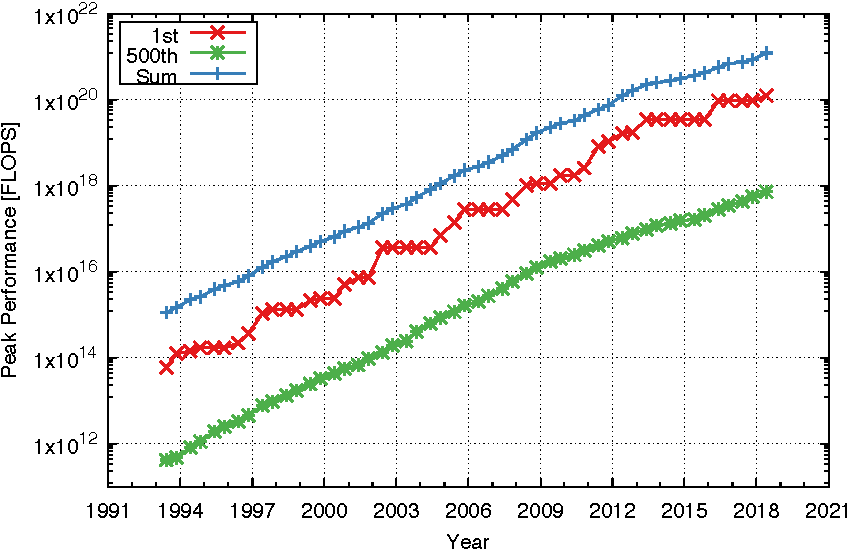
\includegraphics{top500_rmax}
    \caption{Performance Development of Top500 HPC Systems~\autocite{top500}}%
    \label{fig:top500-rmax}
\end{figure}

\subsection{Cluster Architecture}\label{i:cluster-arch}

% クラスタとはなにか
Modern HPC systems mostly adopt \emph{cluster} architecture to achieve their
massive computing performance. In fact, 87\% of the recent Top500 systems
as of July 2018 are based on the cluster architecture. A cluster is an
aggregation of interconnected computers working cooperatively. Computers that
constitute a cluster perform computation in parallel and exchange data to be
required with one another.

% クラスタの構成要素
Figure~\ref{fig:cluster} shows the architectural overview of a typical
cluster. A cluster consists of multiple computers~(\emph{i.e.,\ compute
nodes}), and a high-performance and low-latency network that
integrates~(\emph{i.e.,\ interconnect}) them together as a single system. For
the purpose of sharing input and output data between the compute nodes, a
shared file system is usually deployed as a part of the cluster. Since many
users share a single cluster, a \emph{job scheduler} is also commonly deployed
to efficiently and effectively manage the computing resources in a cluster. A
job scheduler accepts job requests from users and determines when to run each
job to fulfill the request. The scheduler is also responsible for allocating
compute nodes to the job request and launching a job on the allocated nodes.

\begin{figure}
    \centering
    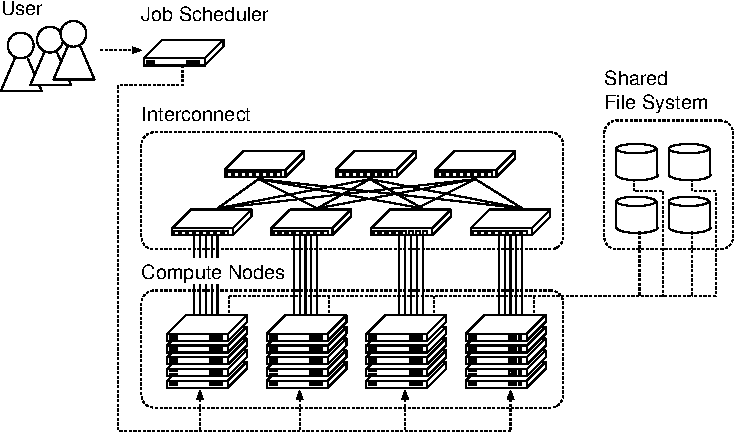
\includegraphics{cluster}
    \caption{Cluster Architecture}%
    \label{fig:cluster}
\end{figure}

% クラスタの規模拡大
The number of compute nodes composing a cluster has a strong trend to
increase. Although the computing performance of a single processor and compute
node have been steadily improving, the growth is not fast enough to meet the
high demand for computing power from the scientists. Therefore, the designers
of HPC systems need to scale out the number of compute nodes to further
improve the total computing performance of the cluster. As a result, a single
cluster accommodates tens of thousands of compute nodes and millions of cores
nowadays.

% 相互結合網の重要性
The bandwidth and latency of communication between compute nodes over the
interconnect, or the communication performance, is essential to the
scalability of the cluster. In general, compute nodes need to frequently
communicate with one another during parallel computation to exchange
intermediate results and control messages. If the communication between
compute nodes becomes a performance bottleneck, simply adding compute nodes to
the cluster does not increase the total performance of the cluster. Therefore,
great efforts have been put to the research and development of
high-performance interconnects.

\subsection{Interconnect}\label{sec:i-interconnect}

% 相互結合網の目的
The main goal of high-performance interconnects is to provide high bandwidth
and low latency in communication between a large number of compute nodes.
In fact, the state-of-the-art interconnects provide more than 100 Gbps
bandwidth and less than 1 $\mu$s latency between tens of thousands of compute
nodes. While achieving such high communication performance, the monetary cost
to build and maintain the interconnect must be reasonable.

% 通信規格
Ethernet~\autocite{Trowbridge2007} and InfiniBand~\autocite{Buyya2009} are
network technology standards commonly utilized for interconnects today.
Ethernet is a long-standing network technology that has been ubiquitously used
in both local area networks and wide are networks. InfiniBand, on the other
hand, is a network standard specifically designed for HPC\@. InfiniBand
offloads most of its protocol stack onto hardware and realizes mechanisms such
as kernel bypassing and Remote Direct Memory Access~(RDMA) to reduces the
communication latency. In addition to Ethernet and InfiniBand, some HPC system
vendors develop proprietary interconnects for their systems. For instance,
Cray has developed Gemini~\autocite{Alverson2010} interconnect and
Aries~\autocite{Faanes2012} interconnect for their systems. Fujitsu has
developed Tofu~\autocite{Ajima2012} interconnect.

% トポロジ
Topology is a key factor that determines the performance of an interconnect.
A fully-connected topology is ideal since it has dedicated links between any
pair of compute nodes. However, implementing a fully-connected topology in a
large scale cluster is unrealistic due to extremely high cost and complexity.
Therefore, various topologies have been proposed to balance the trade-off
between cost and performance. Figure~\ref{fig:topology} illustrates some of
the popular topologies. For example, fat-tree~\autocite{Leiserson1985},
dragonfly~\autocite{Kim2008}, multi-dimensional
torus~\autocite{Alverson2010,Ajima2012}, and hypercube~\autocite{Dally2003} have
been widely adopted as interconnect topologies in HPC systems.

\begin{figure}
    \centering
    \begin{subfigure}{.45\linewidth}
        \centering
        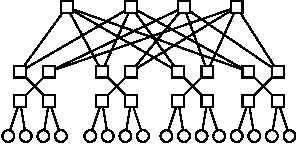
\includegraphics[scale=1.2]{topology-fattree}
        \caption{Fat-tree}%
        \label{fig:topology-fattree}
    \end{subfigure}
    \begin{subfigure}{.45\linewidth}
        \centering
        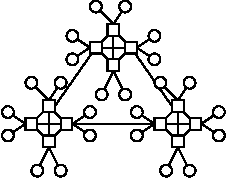
\includegraphics[scale=1.2]{topology-dragonfly}
        \caption{Dragonfly}%
        \label{fig:topology-dragonfly}
    \end{subfigure}
    \par\bigskip
    \begin{subfigure}{.45\linewidth}
        \centering
        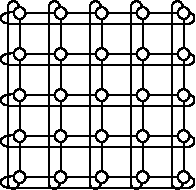
\includegraphics[scale=1.2]{topology-torus}
        \caption{2D Torus}%
        \label{fig:topology-torus}
    \end{subfigure}
    \begin{subfigure}{.45\linewidth}
        \centering
        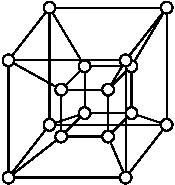
\includegraphics[scale=1.2]{topology-hypercube}
        \caption{4D Hypercube}%
        \label{fig:topology-hypercube}
    \end{subfigure}
    \caption{Topology of Interconnects}%
    \label{fig:topology}
\end{figure}

Mostly, the interconnects of computer cluster systems are full-bisection.
The bisection bandwidth for an interconnect is defined as the minimum
bandwidth between two halves of the interconnect. A full-bisection
interconnect is an interconnect whose bisection bandwidth is larger or equal
to the aggregated bandwidth between compute nodes. Interconnects that are
not full-bisection are referred as oversubscribed. Full-bisection interconnect
design are preferred since such interconnect does not suffer from network
contention even in the worst case scenario where one half of the compute nodes
communicate with the other half at maximum speed of their network interfaces.
This characteristic is beneficial for applications since it removes the need
to be aware of the current contention state of the interconnect. However,
there is a common problem with full-bisection design: the monetary cost to
implement such a design increases superlinearly as the number of node scales
out. Therefore, researches have have worked on the effective utilization of
oversubscribed interconnects~\autocite{Leon2017,Michelogiannakis2017} under
the assumption that oversubscribed interconnects become inevitable in the
future.

\subsection{Message Passing Interface}\label{sec:i-mpi}

% MPIとは
Message Passing Interface~(MPI)~\autocite{MessagePassingInterfaceForum2015} is
a \emph{de facto} standard specification for inter-process communication
libraries used to develop parallel applications running on distributed memory
system such as clusters. MPI defines a suite of communication primitives that
help application developers to build parallel distributed applications that
require complex communications among compute nodes.

% 相互結合網の抽象化
A remarkable feature of MPI is that it abstracts the underlying network
of clusters. As shown in Fig.~\ref{fig:mpi-arch}, each interconnect technology
requires the application developers to use a different set of APIs. MPI hides
this difference and allows application developers to build applications
without forcing them to study the detailed architecture or structure of the
underlying network. For instance, every process is identified by a \emph{rank}
number, a consecutive non-negative integer. The mapping between rank numbers
and network addresses is automatically handled by the MPI library. Every
process belongs to one or more groups of processes, which are called
\emph{communicators}. MPI communication is restricted between processes that
belong to the same communicator. These abstractions make MPI applications
portable and easy to be ported to different clusters.

\begin{figure}
    \centering
    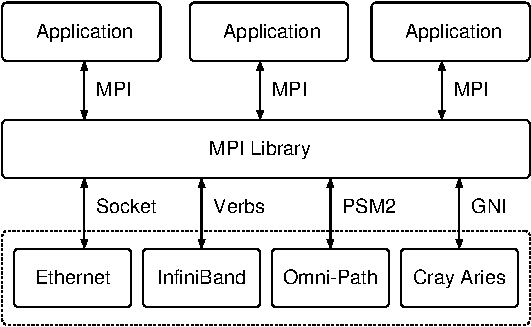
\includegraphics{mpi-arch}
    \caption{Abstraction Provided by MPI}%
    \label{fig:mpi-arch}
\end{figure}

% 1対1通信と集団通信
The communication primitives defined in MPI can be roughly categorized into
point-to-point communication, collective communication and one-sided
communication. Table~\ref{tbl:mpi-primitives} shows several examples from each
category. Note that this list covers only a small fraction of all the
primitives defined in MPI\@.

% 1対1通信
Point-to-point communication is a communication between a sender process and
another receiver process. For example, the sender calls MPI\_Send whereas the
receiver calls MPI\_Recv. It is similar to BSD sockets, but MPI point-to-point
communication differs from sockets in three aspects. First, establishing a
connection between the sender and receiver (\emph{i.e.,} connect, listen,
accept, \emph{etc.}) is not necessary since the MPI library takes care of it
internally. Second, the order of calls to MPI\_Send on the sender side and
MPI\_Recv on the receiver side does not matter due to the internal
buffering mechanism in the MPI library. In contrast, calling the recv function
after the send function when using sockets may result in packet drops. This
characteristic ensures deterministic behavior of applications. Finally, a
\emph{tag} can be associated to each message to indicate the type or context
of the message. In sockets, messages are merely binary sequences without
having any context.

% 集団通信
Collective communication involves a group of processes and provides frequently
used communication patterns by scientists when implementing parallel
algorithms such as broadcast, reduction, all-to-all exchange, \emph{etc.} In
principle, any collective communication can be implemented using a combination
of point-to-point communication. However, the use of collective communication
over the use combinational use of point-to-point communication is generally
preferable because the MPI library implements each communication primitive
based on optimized algorithms that are selected depending on the message size
and number of processes. For instance, a naive implementation of broadcast
where the root process sends the same data to each non-root process requires
$O(n)$ time to complete ($n$ represents the total number of processes). A more
efficient implementation of broadcast is a tree-like data delivery where
non-root processes help the root process by sending the received data to other
processes that have not received the data yet. The time complexity of
tree-like broadcast is $O(\log n)$.

% 同期通信と非同期通信
Both point-to-point communication primitives and collective communication
primitives have blocking and non-blocking versions. Blocking primitives waits
until the communication completes. In contrast, non-blocking primitives
returns immediately after initiating the corresponding communication
operation. A separate synchronization is prepared to complete the
communication. The advantage of non-blocking communication is that it allows
overlapped computation and communication. In other words, computation can be
performed while the communication is in progress. Overlapping computation and
communication is a way to hide the cost of communication and usually results
in better application performance. As a trade-off, non-blocking communication
slightly increases the programming effort compared to blocking communication.

% 片側通信
One-sided communication is a form of Remote Memory Access~(RMA). In
point-to-point communication, the sender and receiver need to mutually agree
to start a communication. In contrast, one-sided communication allows
a process to directly read or write the memory of a peer process without the
involvement of its counterpart. This communication model reduces the overhead
incurred by memory copy and synchronization points. One-sided communication is
especially beneficial on interconnects that support Remote Direct Memory
Access~(RDMA).

\begin{table}
    \centering
    \caption{Examples of MPI Primitives}%
    \label{tbl:mpi-primitives}
\begin{tabular}{@{}lll@{}}
\toprule
Type           & Name        & Description \\ \midrule
Point-to-point & Send/Recv   & Point-to-point send and receive              \\
               & Isend/Irecv & Non-blocking point-to-point send and receive \\
\midrule
Collective     & Bcast       & Broadcast                                    \\
               & Reduce      & Reduction                                    \\
               & Allreduce   & Broadcast result of reduction                \\
               & Ibcast      & Non-blocking Bcast                           \\
               & Ireduce     & Non-blocking Reduce                          \\
               & Iallreduce  & Non-blocking Allreduce                       \\
\midrule
One-sided      & Put         & One-sided put                                \\
               & Get         & One-sided get                                \\
\bottomrule
\end{tabular}
\end{table}

% MPIの実装
There are multiple implementations of the MPI standard. Open
MPI~\cite{Squyres2005}, MPICH~\cite{Gropp2002} and MVAPICH~\cite{mvapich} are
representative examples of
actively developed open source implementations of MPI\@.
Furthermore, HPC system vendors such as Cray, Intel and Fujitsu offer their
own proprietary MPI implementations based upon the open source
implementations, taking the feature and characteristics of their own HPC
systems into consideration. Vendor MPI implementations are highly optimized
for the vendor's HPC system and able to take advantage of the special features
of their system. In addition to the header files and libraries that implement
the APIs defined in the specifications, MPI implementations usually offer a
launcher that allows users to quickly start MPI processes on multiple compute
nodes.

% MPIの高速化
Until today, countless scientific applications have been developed with MPI\@.
Accompanied by the recent scale-out of clusters, the execution time of MPI
primitives has become a critical factor that determines the total performance
of these applications using MPI\@. In other words, the total performance of
MPI applications can be improved by optimizing the performance of MPI
communications. For this reason, researchers have been striving to improve the
communication performance of MPI from various aspects.

\subsection{Problem and Motivation}\label{sec:i-problem}

% アプリケーションの通信パターン
The inter-process communication of MPI applications shows a distinctive
pattern. This pattern varies depending on the application and originates from
the mathematical model, discretization method, and parallelization strategy.
Figure~\ref{fig:stencil3d} shows the communication pattern of a
three-dimensional finite-difference solver that performs the nearest neighbor
communication as an example. In this figure, the total size of messages sent
from a process to another process is visualized using a heat map. The
horizontal axis and vertical axis represent the sender and receiver rank,
respectively. The visual representation evidently exhibits a regular and local
pattern along the diagonal, which originates from the nearest neighbor
communication required by the finite-difference method.

\begin{figure}
    \centering
    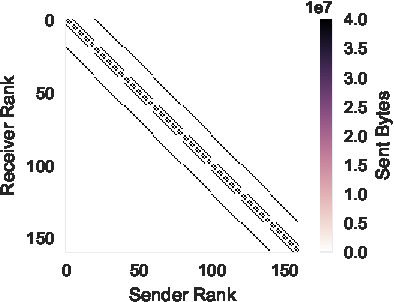
\includegraphics[width=0.6\linewidth]{stencil3d}
    \caption{Communication Pattern of an Application}%
    \label{fig:stencil3d}
\end{figure}

% 相互結合網は通信パターンを無視している
The design of an interconnect could be highly optimized for an
application by taking the communication pattern of applications into account.
For instance, the interconnect with a three-dimensional torus topology would
be ideal for an application that performs nearest neighbor communication in
three-dimensional space. However, this approach is infeasible when designing a
real-world cluster. The reason can be explained from the fact that HPC systems
are shared by many users where each user runs various applications on the
cluster. Therefore, in contrast to the application-dependent communication
pattern, the interconnect is inherently application-independent.

% 問題
As a result, a concentration of packet flow in the interconnect, or the
imbalance of packet flow, can take place under a certain combination of
communication pattern and interconnect. The imbalance can lead to the
concentration of traffic on a link in the interconnect and the slowdown of MPI
communication that uses the link. The degraded MPI communication can
ultimately result in serious degradation of total application performance.

% 関連研究
A  number of previous studies have tried to address the mismatch between
application-dependent communication patterns and application-independent
interconnects. Researchers have attempted to adapt the communication
pattern of applications to the interconnect. For instance, interconnect-aware
MPI collectives~\autocite{Kumar2016,Kumar2014,Gong2015,Adachi2013} have been
developed to improve the performance of MPI collectives by taking the
interconnect of a cluster into account. MPI implementation often leverages
tree-based algorithms to aggregate and distribute messages from and to
processes. Interconnect-aware MPI collectives use the information on the
interconnect, such as topology and link bandwidth, to build a delivery tree
that matches the underlying interconnect of the cluster. Another approach is
to optimize the placement of MPI processes on the compute
nodes~\autocite{Michelogiannakis2017,Hoefler2011,Choi2017}. In this
approach, the communication pattern of an application is considered as a
weighted graph where nodes represent processes and edges represent the volume
of data exchanges between two processes. Various heuristic algorithms have
been proposed to embed the communication pattern graph onto the interconnect
topology.

% 相互結合網の動的制御は未だ研究が進んでいない
To date, however, there has been few studies on adapting the
interconnect to the communication pattern of applications. This is mostly
because it has been assumed that flexibly and dynamically reconfiguring the
interconnect at run-time is infeasible. However, this assumption might not hold
anymore with the recent emergence of programmable networking architecture that
allows the on-the-fly reconfiguration of the interconnect.

\subsection{Software-Defined Networking}\label{sec:i-sdn}

% SDN
Software-Defined Networking (SDN) is a novel networking architecture
that separates the control plane and data plane into different devices.
In conventional networking architectures, the decision on how to handle
packets (control plane) and the packet transfer (data plane) are
implemented as unified and inseparable features. The separation of the
control plane and data plane allows SDN to deliver the following three
benefits:

\begin{enumerate}
\item
  \emph{Programmable}: The control plane can be handled by a software
  controller. Network operators develop software controllers tailored for
  their needs.
\item
  \emph{Dynamic}: SDN allows the controller to quickly reconfigure the
  network. For instance, it is possible to dynamically optimize packet
  flows in the network based on the real-time traffic pattern.
\item
  \emph{Centralized}: A centralized controller configures the entire
  SDN-enabled network, thus reducing efforts to administer and manage
  the network. In conventional networking architectures, the operators
  need to configure each network device separately because the control
  plane is distributed on individual devices.
\end{enumerate}

\begin{figure}
    \centering
    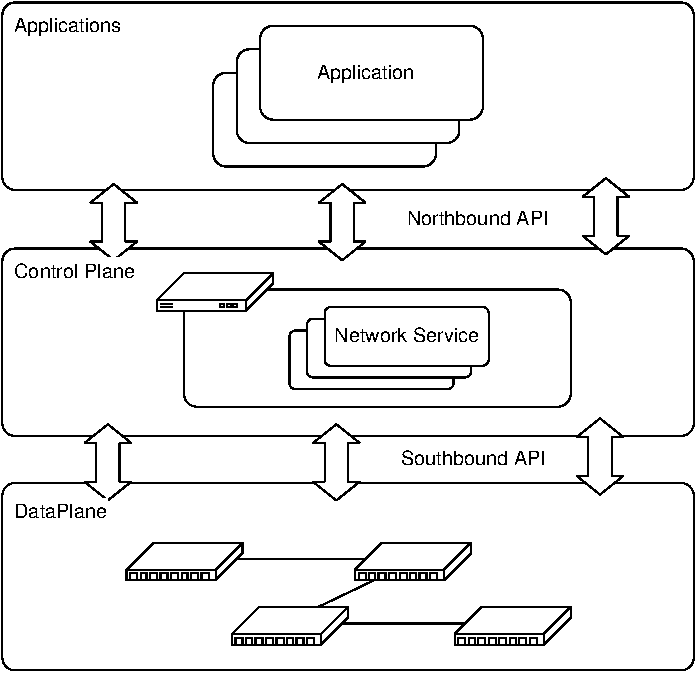
\includegraphics{sdn}
    \caption{Software-Defined Networking Architecture}%
    \label{fig:sdn-architecture}
\end{figure}

% OpenFlowの概要とスイッチ
\emph{OpenFlow}~\autocite{McKeown2008} is a widely accepted open standard of
SDN\@. In an OpenFlow-enabled network, the data plane is handled by OpenFlow
switches. Each OpenFlow switch holds a logical construct called a \emph{flow
table}, which is a collection of \emph{flow entries}. A flow entry defines
what kind of packet control should be performed on what kind of packets
(Fig.~\ref{tbl:flow-table}). Every time a packet arrives at an OpenFlow
switch, the switch looks up a matching flow entry in its flow table using the
header fields of the packet. Once the switch finds a matching flow entry, the
corresponding action of the matched flow entry is applied to the incoming
packet. An arbitrary combination of pre-defined header fields can be used for
the matching condition. Table~\ref{tbl:flow-fields} shows the twelve header
fields defined in OpenFlow~1.0. OpenFlow switches usually implement
specialized hardware such as Content Addressable Memory (CAM) or Ternary
Content Addressable Memory (TCAM) to perform the matching efficiently.

\begin{figure}
\centering
\begin{tabular}{@{}lllll@{}}
\toprule
\multicolumn{3}{c}{Matching Condition} & \multirow{2}{*}{Action} \\ \cmidrule(){1-3}
Dst MAC     & Src     & Dst IP    &                         \\ \midrule
                  & 192.0.2.12 & 192.0.2.34  & Output to port 1         \\
                  & 192.0.2.34 & 192.0.2.56  & Output to port 2         \\
ff:ff:ff:ff:ff:ff &            &             & Output to port 1 and 2   \\
72:42:c1:e4:75:8c &            &             & Drop                     \\
\bottomrule
\end{tabular}
\caption{An Example of a Flow Table}%
\label{tbl:flow-table}
\end{figure}

\begin{table}
\centering
\caption{Header Fields Defined in OpenFlow 1.0}%
\label{tbl:flow-fields}
\begin{tabular}{@{}llr@{}}
\toprule
Layer               & Field Name               & Width (bits) \\ \midrule
L1                  & Ingress Port             &              \\ \cmidrule(l){2-3}
\multirow{5}{*}{L2} & Ethernet Source          & 48           \\
                    & Ethernet Destination     & 48           \\
                    & Ethernet Type            & 16           \\
                    & VLAN ID                  & 12           \\
                    & VLAN Priority            & 3            \\ \cmidrule(l){2-3}
\multirow{4}{*}{L3} & IP Source                & 32           \\
                    & IP Destination           & 32           \\
                    & IP Protocol              & 8            \\
                    & IP ToS                   & 6            \\ \cmidrule(l){2-3}
\multirow{2}{*}{L4} & TCP/UDP Source Port      & 16           \\
                    & TCP/UDP Destination Port & 16           \\ \bottomrule
\end{tabular}
\end{table}

% コントローラ
The OpenFlow controller is a component responsible for the control plane. It
manages the flow table of each switch by adding, modifying and removing flow
entries. The controller and switches communicate with each other by
asynchronously exchanging messages defined in the OpenFlow protocol
specification. Table~\ref{tbl:openflow-messages} shows a list of message types
defined in OpenFlow~1.0. In this table, messages are classified into three
categories by its initiator. Controller-initiated messages are used by the
controller to update or inspect the state of a switch. On the other hand,
switch-initiated messages are used by switches to notify the controller of
network events and update in the switch state. Symmetric messages are
initiated from both sides and used primarily for establishing and maintaining
the connection between the controller and switch. Messages may or may not
require a response from its receiver depending upon the message type. One of
the most frequently used message type is \emph{packet-in}, which is sent out
from a switch to the controller when a matching flow entry is missing for an
incoming packet. In response, the controller can send a \emph{modify flow
entry} message to install a new flow entry on the switch.

% コントローラフレームワーク
OpenFlow controllers are usually implemented as a software for flexibility and
reduced development cost. OpenFlow controller frameworks have been developed
to support the developments of OpenFlow controller software by providing
reusable building blocks. Common building blocks include parser and deparser
of OpenFlow messages and common network protocol packets, state machine for
the OpenFlow protocol and high-performance concurrent server for handling the
connection with the switches. Trema~\autocite{trema}, Ryu~\autocite{Ryu2014},
ONOS~\autocite{Berde2014} and OpenDaylight~\autocite{Medved2014} are among the
most popular OpenFlow controller frameworks. Developers of OpenFlow
controllers can focus to the application logic by taking advantage of these
controller frameworks.

\begin{table}[t]
\centering
\caption{Messages Types Defined in OpenFlow 1.0}%
\label{tbl:openflow-messages}
\begin{tabular}{@{}llcl@{}}
\toprule
Initiator                   & Message Type     & Response     & Purpose                               \\ \midrule
\multirow{9}{*}{Controller} & Packet-Out       &              & Inject a packet to data plane         \\
                            & Flow-Mod         &              & Add/Modify/Delete a flow entry        \\
                            & Port-Mod         &              & Modify state of a port                \\
                            & Stats            & $\checkmark$ & Get statistics of individual flow     \\
                            & Barrier          & $\checkmark$ & Synchronize controller and switch     \\
                            & Queue-Get-Config & $\checkmark$ & Query state of queues                 \\
                            & Features         & $\checkmark$ & Get capabilities of switch            \\
                            & Get-Config       & $\checkmark$ & Get fragmentation setting of switch   \\
                            & Set-Config       &              & Set fragmentation setting of switch   \\ \midrule
\multirow{3}{*}{Switch}     & Packet-In        &              & Notify an unmatched packet            \\
                            & Flow-Removed     &              & Notify when a flow entry been removed \\
                            & Port-Status      &              & Notify status update of a port        \\ \midrule
\multirow{4}{*}{Symmetric}  & Hello            &              & Negotiate OpenFlow version            \\
                            & Error            &              & Notify failure                        \\
                            & Echo             & $\checkmark$ & Check liveness of connection          \\
                            & Vendor           &              & Vendor-specific extensions            \\ \bottomrule
\end{tabular}
\end{table}

\clearpage

\section{Research Objective}\label{sec:i-objective}

As discussed in Section~\ref{sec:i-problem}, the mismatch between
application-dependent communication patterns and application-independent
interconnects have led to the imbalance of packet flow in the interconnect.
This dissertation aims to address this imbalance problem by establishing a
programmable interconnect control that dynamically controls the packet flow in
the interconnect based on the communication pattern of applications.

\begin{figure}
    \centering
    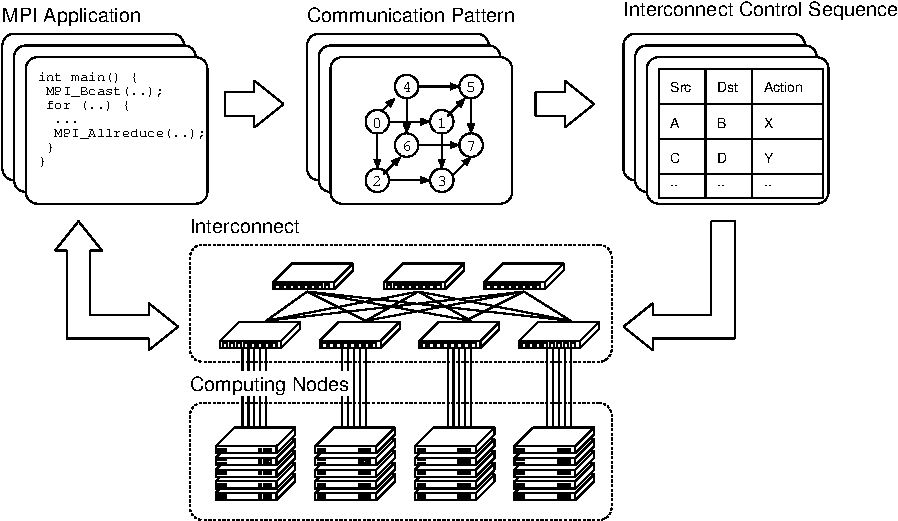
\includegraphics{objective}
    \caption{Concept of the Envisioned Programmable Interconnect Control}%
    \label{fig:objective}
\end{figure}

Figure~\ref{fig:objective} illustrates the high-level concept of the
envisioned programmable interconnect control in this dissertation. The core
idea of this programmable interconnect control is an iteration of three steps:
\emph{observe}, \emph{decide} and \emph{adapt}. The envisioned interconnect
control functions as follows. First, the inter-process communication pattern
of an application is observed and recorded. Second, the decision on how to
control the packet flow in the interconnect is made based on the collected
communication pattern of the application. The goal of this packet flow control
is to mitigate load imbalance in the interconnect and achieve higher
communication performance between compute nodes. Third, the interconnect is
adapted to perform the planned packet flow control using programmable
networking architecture. These three steps are performed in synchronization
with the execution of application.

To materialize this concept, the following three challenges must be achieved:

\begin{enumerate}
\item \emph{Analyzing the packet flow in the interconnect}:
    To effectively control the packet flow in the interconnect, interconnect
    designers first need to carefully analyze and understand the packet flow
    generated in the interconnect when running an application on a cluster.
\item \emph{Accelerating MPI communication by dynamically controlling the
    packet flow in the interconnect}:
    Given a communication pattern of an application and an interconnect,
    interconnect designers need to determine how to control the packet flow in
    the interconnect to mitigate load imbalance in the interconnect and
    improve the performance of MPI communication.
\item \emph{Coordinating the execution of application and interconnect control}:
    The communication pattern of the application changes rapidly with the
    execution of the application. Therefore, the interconnect control must
    be performed in accordance with the execution of application.
\end{enumerate}

\section{Organization of the Dissertation}

The rest of this dissertation is organized as follows.
% アプリケーションが相互結合網内に生成するパケットフローの解析手段を実現
Chapter~\ref{sec:ii} proposes PFAnalyzer, a toolset for analyzing the
packet flow in the interconnect, to address the first challenge listed in
Section~\ref{sec:i-objective}. The packet flow generated in the interconnect
highly depends on parameters such as the communication pattern of application,
interconnect design and cluster configuration. When designing and implementing
an efficient programmable interconnect control, researchers need to conduct a
systematic analysis over many combinations of these parameters. Since
performing such analysis on a physical cluster is time-consuming, this
dissertation utilizes simulation to facilitate the analysis. PFAnalyzer is a
pair of two tools: PFSim, an interconnect simulator specialized for
programmable interconnects, and PFProf, a profiler to collect communication
pattern from MPI applications. PFSim allows interconnect researchers and
designers to investigate possible congestion in the interconnect for an
arbitrary cluster configuration and a set of communication patterns collected
by PFProf. This dissertation evaluates the accuracy of the simulation results
obtained from PFSim and demonstrates how PFAnalyzer can be used to analyze the
effect of programmable interconnect control.

% MPI集団通信を高速化するパケットフロー制御アルゴリズムを配備可能な
% フレームワークを構築
Chapter~\ref{sec:iii} addresses the second challenge. Out of the communication
primitives provided by MPI, this dissertation focuses on accelerating
collective communication because it occupies a significant fraction of the
execution time of applications. This dissertation proposes a framework to
accelerate MPI collectives by dynamically controlling the packet flow in the
interconnect. The network programmability provided by Software-Defined
Networking is integrated into MPI collectives so that collectives are able to
effectively utilize the bandwidth of the interconnect. In particular, this
dissertation aims to reduce the execution time of MPI\_Allreduce, which is a
frequently used MPI collective communication in many simulation codes. The
speedup of MPI\_Allreduce when using the proposed collective acceleration
framework is evaluated.

% 通信と計算が連係動作する新たなクラスタアーキテクチャを確立
Chapter~\ref{sec:iv} addresses the third challenge. This chapter proposes
UnisonFlow, a software-defined coordination mechanism that performs
interconnect control in synchronization with the execution of applications.
In a real-world application, the communication pattern changes with the
execution of application. Therefore, a mechanism to coordinate packet flow
control and execution of application is essential. UnisonFlow is a
kernel-assisted mechanism that realizes such coordination on a per-packet
basis while maintaining significantly a low overhead. Evaluation verifies that
the interconnect control can be successfully performed in synchronization with
the execution of the application and the overhead incurred by the coordination
mechanism is small.

Chapter~\ref{sec:v} concludes this dissertation and discusses future works.
